% ======================================================================
%  SHEO — client presentation deck (compiled with tectonic / XeLaTeX)
%  Modern, minimal beamer theme. Self-contained — no external theme pkgs.
%  Figures are shared with the report (../report/figures).
% ======================================================================
\documentclass[aspectratio=169,11pt]{beamer}

\usepackage{fontspec}
\usepackage{graphicx}
\usepackage{booktabs}
\usepackage{amssymb}
\usepackage{tikz}
\usetikzlibrary{positioning,arrows.meta,fit,backgrounds}
\usepackage{xcolor}
\graphicspath{{figures/}{../report/figures/}}

% ---- palette (matches the report figures: Okabe–Ito) ----
\definecolor{accent}{HTML}{0072B2}
\definecolor{accent2}{HTML}{D55E00}
\definecolor{green}{HTML}{009E73}
\definecolor{ink}{HTML}{1A1A1A}
\definecolor{mut}{HTML}{6E7781}
\definecolor{card}{HTML}{F4F7FA}
\definecolor{cardbd}{HTML}{D7E3EE}

% ======================================================================
%  Minimal modern theme
% ======================================================================
\usefonttheme{professionalfonts}
\setbeamercolor{normal text}{fg=ink}
\setbeamercolor{structure}{fg=accent}
\setbeamercolor{frametitle}{fg=accent}
\setbeamercolor{itemize item}{fg=accent}
\setbeamercolor{itemize subitem}{fg=mut}
\setbeamercolor{block title}{fg=white,bg=accent}
\setbeamercolor{block body}{fg=ink,bg=card}
\setbeamerfont{frametitle}{series=\bfseries,size=\Large}
\setbeamerfont{title}{series=\bfseries}
\setbeamertemplate{navigation symbols}{}
\setbeamertemplate{itemize item}{\small\raisebox{0.5pt}{\textbullet}}
\setbeamertemplate{itemize items}[circle]
\setbeamertemplate{blocks}[rounded][shadow=false]

% frametitle: title + thin accent rule beneath
\setbeamertemplate{frametitle}{%
  \vspace{0.6em}%
  \begin{beamercolorbox}[wd=\paperwidth,leftskip=0.9cm,rightskip=0.9cm]{frametitle}%
    \usebeamerfont{frametitle}\insertframetitle\par%
    \vspace{2pt}{\color{accent}\rule{0.55\paperwidth}{1.4pt}}%
  \end{beamercolorbox}%
  \vspace{0.2em}%
}

% minimal footline: short title · author · page
\setbeamertemplate{footline}{%
  \hbox{}\vspace{1pt}%
  \hbox to\paperwidth{\hspace{0.9cm}%
    {\color{mut}\scriptsize SHEO — Smart Home Energy Optimizer}%
    \hfill{\color{mut}\scriptsize\insertframenumber}%
    \hspace{0.9cm}}\vspace{4pt}%
}
\setbeamersize{text margin left=0.9cm,text margin right=0.9cm}

% ---- framed screenshot: thin card border, width-fit with a height cap ----
\newcommand{\shot}[2]{{\setlength{\fboxsep}{0pt}\setlength{\fboxrule}{0.6pt}%
  \fcolorbox{cardbd}{white}{\includegraphics[width=\linewidth,height=#1\textheight,keepaspectratio]{#2}}}}

% ---- small helper macros ----
\newcommand{\kw}[1]{\textcolor{accent}{\textbf{#1}}}
\newcommand{\vnd}[1]{\textcolor{green}{\textbf{#1}}}
\newcommand{\when}{\textcolor{accent}{\textsc{when}}}
\newcommand{\thn}{\textcolor{accent2}{\textsc{then}}}

% pill / tag
\newcommand{\pill}[2]{\tikz[baseline=-0.6ex]\node[fill=#1!15,draw=#1,rounded corners=3pt,
  inner xsep=5pt,inner ysep=2pt,font=\scriptsize\bfseries,text=#1!75!black]{#2};}

% feature card for the "at a glance" slide
\newcommand{\fcard}[2]{%
  \begin{beamercolorbox}[wd=0.96\textwidth,sep=6pt,rounded=true]{block body}%
    {\color{accent}\bfseries\small #1}\par\vspace{1pt}{\footnotesize #2}%
  \end{beamercolorbox}}

% ======================================================================
\begin{document}

% ============================ TITLE ============================
{
\setbeamertemplate{footline}{}
\begin{frame}[plain]
  \vfill
  {\color{accent}\rule{\textwidth}{1.6pt}}\par\vspace{0.7em}
  {\Huge\bfseries AI-Driven Smart Home\\[2pt]Energy Optimizer}\par
  \vspace{0.5em}
  {\large\color{mut} A capability-driven home-energy platform with explainable
   automation\\ and bill-saving estimated in Vietnamese đồng}\par
  \vspace{0.5em}{\color{accent}\rule{\textwidth}{1.6pt}}
  \vfill
  {\small\color{mut} Product walkthrough \quad·\quad Hanoi University of Science and Technology}
  \vfill
\end{frame}
}

% ============================ THE BRIEF ============================
\begin{frame}{What you asked for}
  \vspace{0.3em}
  Four things shaped the product. We built to each.
  \vspace{0.8em}

  \begin{columns}[T]
  \column{0.5\textwidth}
    \begin{itemize}\setlength\itemsep{0.7em}
      \item \kw{Many device types}, each with its own controls — without a hand-coded
            screen per device.
      \item \kw{Automation} a resident \emph{may} set; if they don't, the system should
            find the habit and suggest the rule.
    \end{itemize}
  \column{0.5\textwidth}
    \begin{itemize}\setlength\itemsep{0.7em}
      \item A \kw{mock device} stack, since no physical hardware was available.
      \item \emph{The priority:} let the customer \kw{see the bill they save} from a
            suggested rule — in real money.
    \end{itemize}
  \end{columns}

  \vspace{1.0em}
  \begin{center}
  {\color{mut}\small Everything that follows is a working, end-to-end answer to these four points.}
  \end{center}
\end{frame}

% ============================ AT A GLANCE ============================
\begin{frame}{The product at a glance}
  \vspace{0.2em}
  \begin{columns}[T]
  \column{0.5\textwidth}
    \fcard{Live monitoring}{Per-device power, energy in kWh, top consumers — refreshed within seconds.}\par\smallskip
    \fcard{Capability-driven control}{Controls render themselves from each device's own capability description.}\par\smallskip
    \fcard{Explainable rules}{Readable \texttt{WHEN–THEN} automation with conflict checks and an audit log.}
  \column{0.5\textwidth}
    \fcard{Habit recommendations}{Mined from real usage, ranked by saving, accepted only on your say-so.}\par\smallskip
    \fcard{Bill-saving in VND}{Every rule shows its monthly saving \emph{before} you commit, then tracks it.}\par\smallskip
    \fcard{Safe by default}{Auto-action is opt-in, undoable, never powers off a safety-critical device.}
  \end{columns}
\end{frame}

% ============================ MONITORING ============================
\begin{frame}{Live monitoring}
  \begin{columns}[c]
  \column{0.40\textwidth}
    \begin{itemize}\setlength\itemsep{0.6em}
      \item Instantaneous power \kw{per device}, refreshed within seconds.
      \item Energy in \kw{kWh} for today, the billing cycle, and any range.
      \item \kw{Top consumers} ranked by day, week, month.
      \item A silent device is marked \pill{accent2}{offline} after 60\,s and dropped
            from the live total.
    \end{itemize}
  \column{0.60\textwidth}
    \shot{0.74}{shot-dashboard.png}
  \end{columns}
\end{frame}

% ============================ CONTROL ============================
\begin{frame}{Capability-driven control}
  \begin{columns}[c]
  \column{0.42\textwidth}
    No hard-coded screen per device. The back-end publishes a \kw{capability
    description}; the app renders the right control:
    \vspace{0.3em}
    \begin{itemize}\setlength\itemsep{0.25em}
      \item \pill{accent}{toggle} on / off
      \item \pill{accent}{range} fan speed, target temperature
      \item \pill{accent}{enum} mode
    \end{itemize}
    \vspace{0.3em}
    Each command is \kw{validated} and returns
    \pill{green}{success}, \pill{accent2}{rejected}, or \pill{mut}{timeout}.
    \par\vspace{0.2em}
    {\small\color{mut} A new device type needs no new control code.}
  \column{0.58\textwidth}
    \shot{0.80}{shot-devices.png}
  \end{columns}
\end{frame}

% ============================ RULES ============================
\begin{frame}{Explainable automation rules}
  \vspace{0.2em}
  Each rule reads as \when\ \emph{a condition} \thn\ \emph{an action}, over
  \kw{time, day, tariff, state or sensor} — with conflict-flagging and an immutable
  audit log.
  \vspace{0.4em}
  \begin{center}\shot{0.58}{shot-rules.png}\end{center}
\end{frame}

% ============================ RECOMMENDATIONS ============================
\begin{frame}{Habit recommendations}
  \vspace{0.2em}
  When no rule exists, the system \kw{mines the habit} from \kw{7+ days} of usage and
  offers a readable rule with a \kw{rationale} and a ranked \vnd{VND saving} ---
  \kw{advisory} until \emph{Accept}.
  \vspace{0.4em}
  \begin{center}\shot{0.58}{shot-recommendations.png}\end{center}
\end{frame}

% ============================ SAVINGS (the priority) ============================
\begin{frame}{The priority: bill saving in real money}
  \vspace{0.2em}
  \begin{columns}[T]
  \column{0.55\textwidth}
    The customer must \kw{see the money saved} by a suggested rule.
    \vspace{0.4em}
    \begin{itemize}\small\setlength\itemsep{0.45em}
      \item A 14-day \kw{baseline} per device sets the reference.
      \item Saving $=\ \sum\,(\text{baseline}-\text{expected})\times\text{tariff}$ —
            \kw{transparent}, not a black box.
      \item The \vnd{monthly VND estimate} shows \emph{before} you save a rule or accept
            a recommendation.
      \item The \vnd{accrued saving} this cycle is tracked, and a rule is re-checked if
            reality drifts $\pm20\%$.
    \end{itemize}
  \column{0.45\textwidth}
    \vspace{1.2em}
    \begin{beamercolorbox}[wd=\textwidth,sep=12pt,rounded=true]{block body}
      \centering
      {\small\color{mut}Suggested rule}\\[4pt]
      {\bfseries Turn off TV plug at 19:00}\\[10pt]
      {\small\color{mut}Estimated monthly saving}\\[2pt]
      {\Huge\vnd{$\approx$\,38\,000\,₫}}\\[6pt]
      {\scriptsize\color{mut}shown before you accept}
    \end{beamercolorbox}
  \end{columns}
\end{frame}

% ============================ ROLES ============================
\begin{frame}{One building, clear roles}
  \vspace{0.3em}
  The platform models a whole apartment building, with access scoped by role.
  \vspace{0.8em}
  \begin{columns}[T]
  \column{0.5\textwidth}
    \begin{beamercolorbox}[wd=\textwidth,sep=9pt,rounded=true]{block body}
      {\color{accent}\bfseries Administrator} — building owner\par\vspace{3pt}
      \small Read-only overview of every unit, sets the building tariff, onboards or
      offboards residents. Never operates a unit's devices, sees no resident's
      on/off state.
    \end{beamercolorbox}
  \column{0.5\textwidth}
    \begin{beamercolorbox}[wd=\textwidth,sep=9pt,rounded=true]{block body}
      {\color{accent}\bfseries Resident} — tenant of one unit\par\vspace{3pt}
      \small Sees only their own unit. Controls its devices, authors rules, accepts or
      dismisses recommendations, sees their own savings.
    \end{beamercolorbox}
  \end{columns}
  \vspace{0.9em}
  \begin{center}\small\color{mut}
  Authentication and role-based access throughout; a resident can never read another
  unit's data.
  \end{center}
\end{frame}

% ============================ SAFETY / TRUST ============================
\begin{frame}{Safe and trustworthy by design}
  \vspace{0.4em}
  The system \kw{advises and estimates}, but acts on devices only with explicit consent.
  \vspace{0.9em}
  \begin{columns}[T]
  \column{0.5\textwidth}
    \begin{itemize}\setlength\itemsep{0.7em}
      \item Automatic action is \kw{off by default} — opt in per rule.
      \item Every auto-applied action has a \kw{2-minute undo}.
    \end{itemize}
  \column{0.5\textwidth}
    \begin{itemize}\setlength\itemsep{0.7em}
      \item A safety-critical device is \kw{never auto powered off}.
      \item Compressor and out-of-range commands are \kw{rate-limited and rejected}.
    \end{itemize}
  \end{columns}
  \vspace{1.0em}
  \begin{center}
  {\color{mut}\small Deleting a rule keeps its history; nothing happens silently.}
  \end{center}
\end{frame}

% ============================ UNDER THE HOOD ============================
\begin{frame}{Under the hood (briefly)}
  \begin{columns}[c]
  \column{0.46\textwidth}
    \begin{itemize}\setlength\itemsep{0.55em}
      \item \kw{FastAPI} back-end; \kw{React} single-page app over REST + a live
            WebSocket feed.
      \item A \kw{capability schema} is the single source of truth for UI rendering
            \emph{and} command validation.
      \item A deterministic \kw{mock simulator} stands in for hardware — end-to-end and
            hardware-ready.
      \item \kw{67 automated tests} across monitoring, control, rules, savings, safety
            and access control.
    \end{itemize}
  \column{0.54\textwidth}
    \centering
    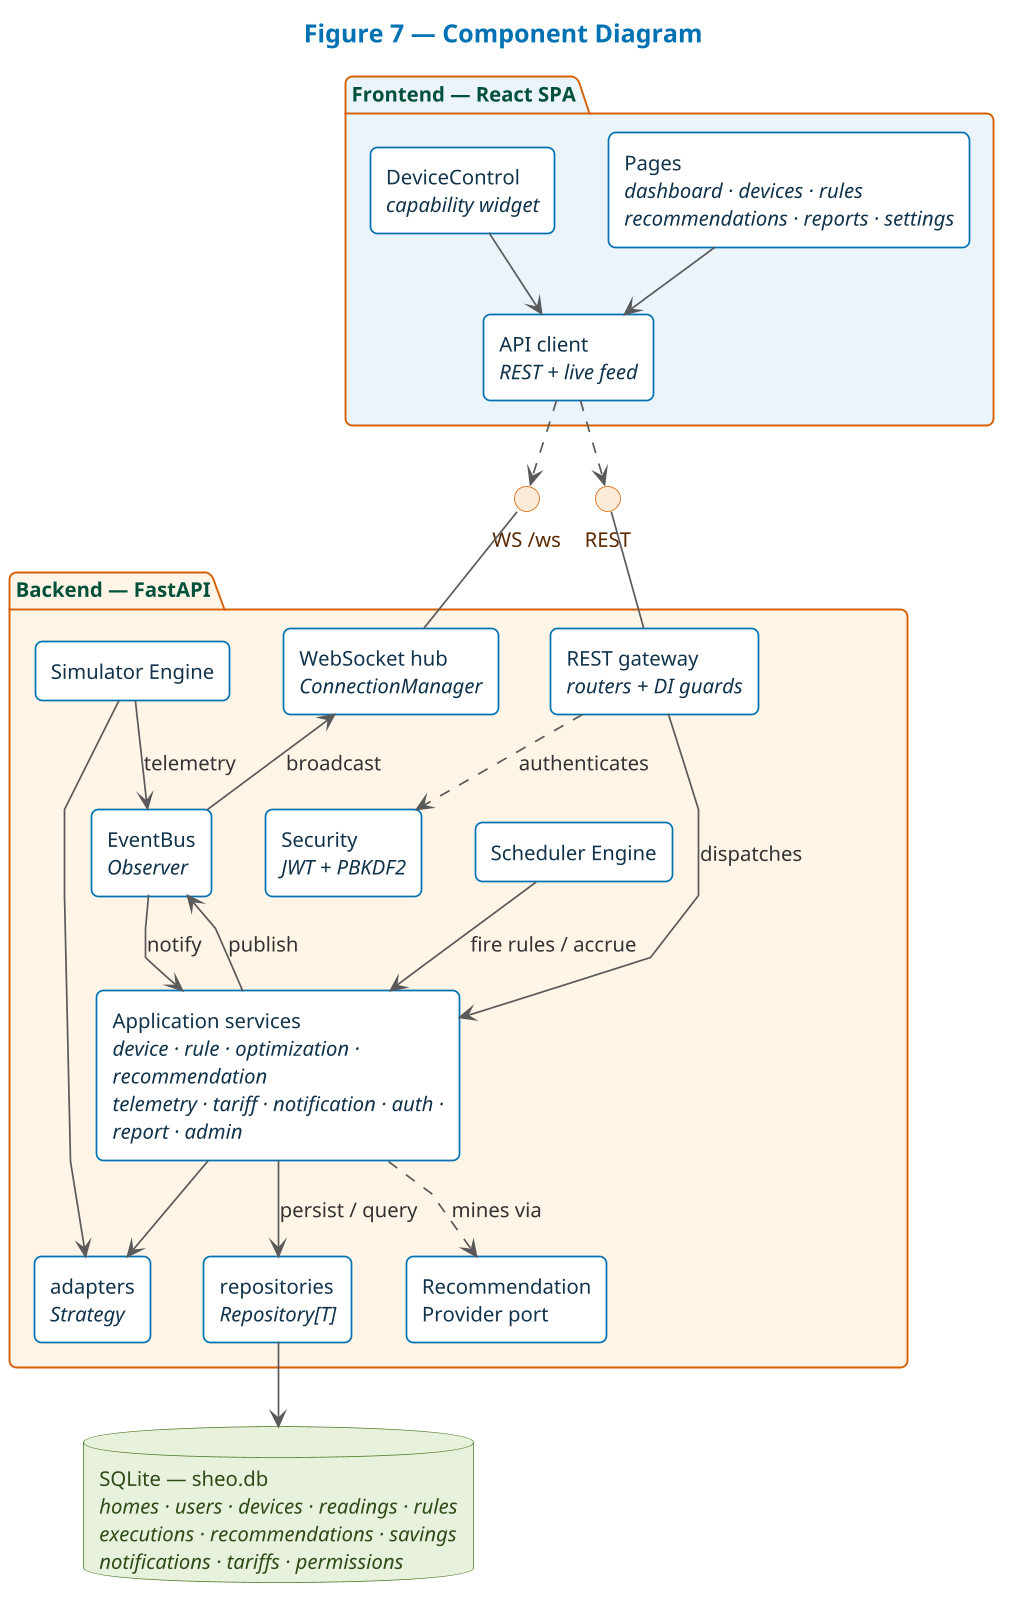
\includegraphics[width=\linewidth,height=0.74\textheight,keepaspectratio]{fig07-component.png}
  \end{columns}
\end{frame}

% ============================ CLOSE ============================
\begin{frame}{Delivered against the brief}
  \vspace{0.4em}
  \begin{columns}[T]
  \column{0.52\textwidth}
    \begin{itemize}\setlength\itemsep{0.65em}
      \item[\textcolor{green}{$\checkmark$}] Controls driven by each device's own capability.
      \item[\textcolor{green}{$\checkmark$}] Habits mined and suggested as readable rules.
      \item[\textcolor{green}{$\checkmark$}] Full mock-device stack, hardware-ready.
      \item[\textcolor{green}{$\checkmark$}] Bill saving shown in \vnd{VND}, before you commit.
    \end{itemize}
  \column{0.48\textwidth}
    \vspace{0.3em}
    \begin{beamercolorbox}[wd=\textwidth,sep=12pt,rounded=true]{block body}
      \centering
      {\color{accent}\bfseries\large Ready for your walkthrough}\\[6pt]
      {\small\color{mut} We'll demonstrate any function live.}
    \end{beamercolorbox}
  \end{columns}
  \vfill
  \begin{center}{\large\bfseries\color{accent} Thank you}\end{center}
  \vspace{0.3em}
\end{frame}

\end{document}
